\documentclass[14pt]{article}
\usepackage{graphicx}
\usepackage[left=3cm, right=1.5cm, top=1.5cm, bottom=2cm]{geometry}
\usepackage[russian]{babel}
\usepackage[T2A]{fontenc}
\usepackage[utf8]{inputenc}
\usepackage[unicode]{hyperref}
\usepackage{a4wide}

\begin{document}
\thispagestyle{empty}
\begin{center}
	\ \vspace{-4cm}\\
	
\includegraphics[width=0.5\textwidth]{../img/msu.png}\\
	{\scshape Московский государственный университет имени М.~В.~Ломоносова}\\
	Факультет вычислительной  математики и кибернетики\\
	\vfill
	{\LARGE Задание по системам управления проектами}\\
	\vspace{1cm}
	{\Huge\bfseries <<Работа в MS Project>>}\\
	{\Huge Вариант 5} 
\end{center}
\vspace{1cm}
\begin{flushright}
	\large
	\textit{Задание выполнил}\\
	Гусейнов Али Эльшанович\\
	\vspace{5mm}
	\textit{Преподаватель}\\
	Абрамов Владимир Геннадьевич
\end{flushright}
\vfill
\begin{center}
	Москва, 2024
\end{center}
\clearpage
\tableofcontents
\clearpage
\section{Команда}
\section{Ресурсы}
	\subsection{Сетевой график}
	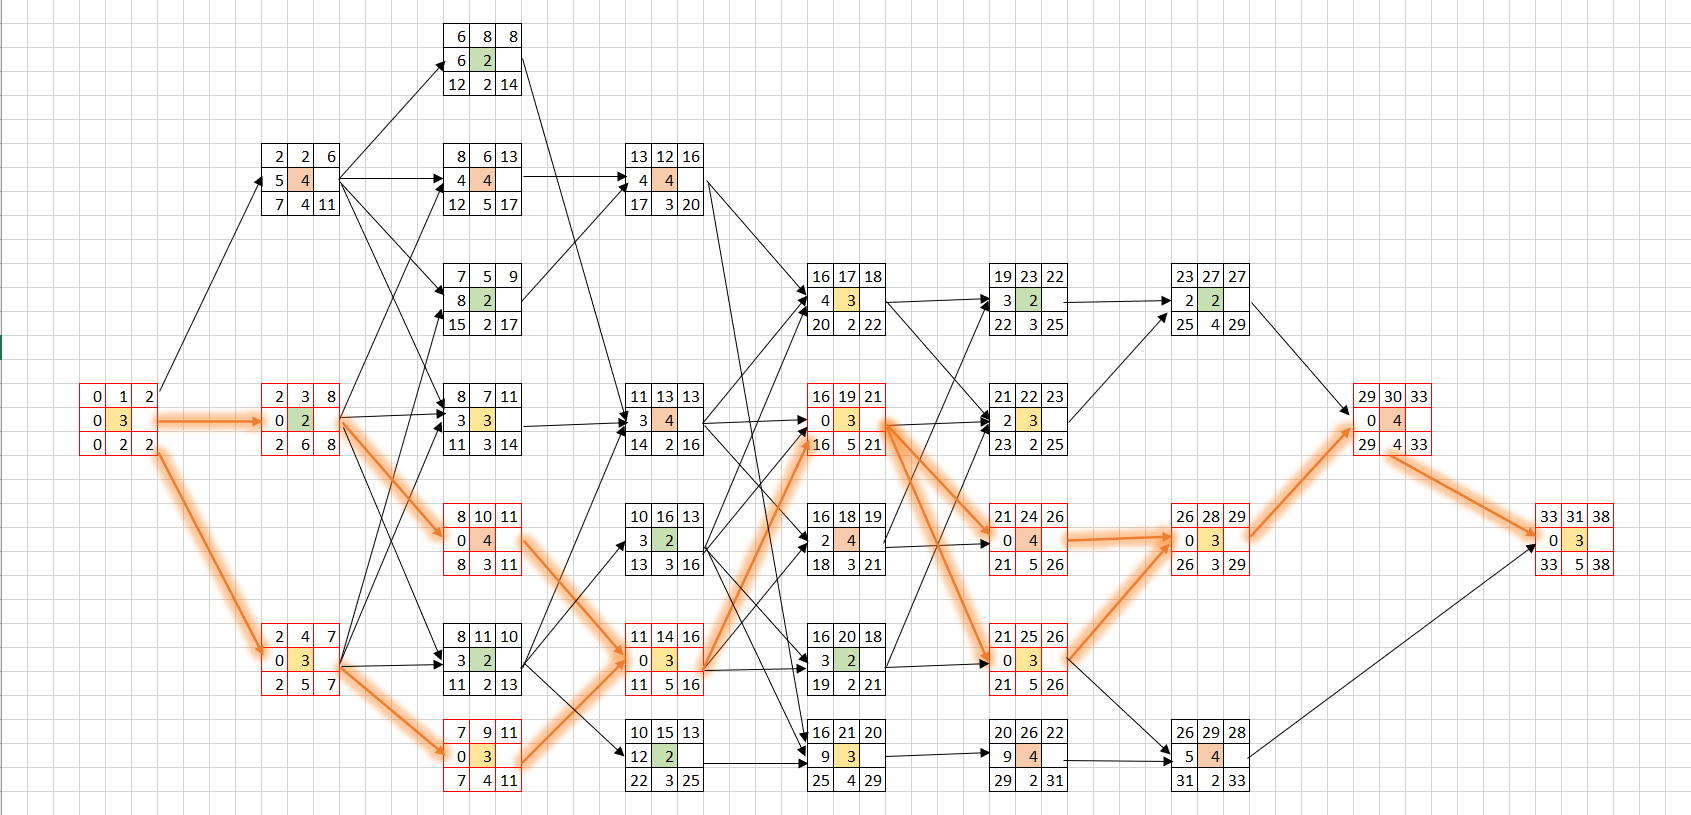
\includegraphics[width=\textwidth]{../img/init_network_graph.png}\\
	В проекте 2 кретических пути.
	\subsection{Назначение ресурсов}
	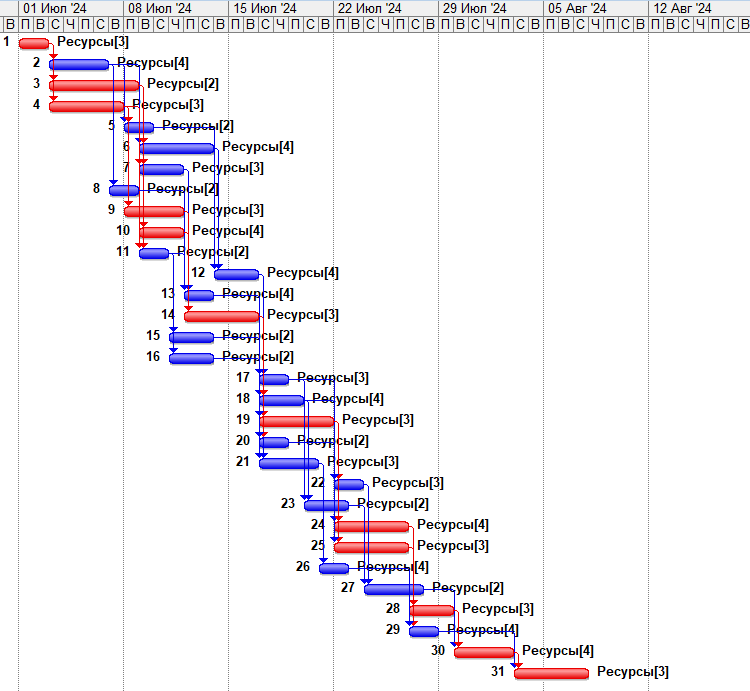
\includegraphics[width=\textwidth]{../img/init_resource_manage.png}
\section{Задача}
	Попробовать уменьшить количество используемых ресурсов до 5 в день, меняя при этом длительность работ не более чем на 2 дня.
\section{Решение}
	Проанализируем поставленную задачу.
	Скопируем данные с \texttt{MS Office Project} в \texttt{Excel} и найдём самое раннее начало,
		самый поздний конец и суммарное количество ресурсов.
	С помощью полученных данных высчитаем колько в среднем в день нужно потратить ресурсов.
	По картинке видно,
		что при таких длительностях с помощью простых отсрочек работ необходимо затрачивать хотя бы 9 ресурсов в день.
	А если утверждать, что параллельно первой и последней работе не может реализовываться ещё один какой-нибудь процесс,
		то необходимо хотя бы 10 ресурсов в день затрачивать, чтобы успеть всё выполнить.
	Требуется уменьшить это число до 5.\\
	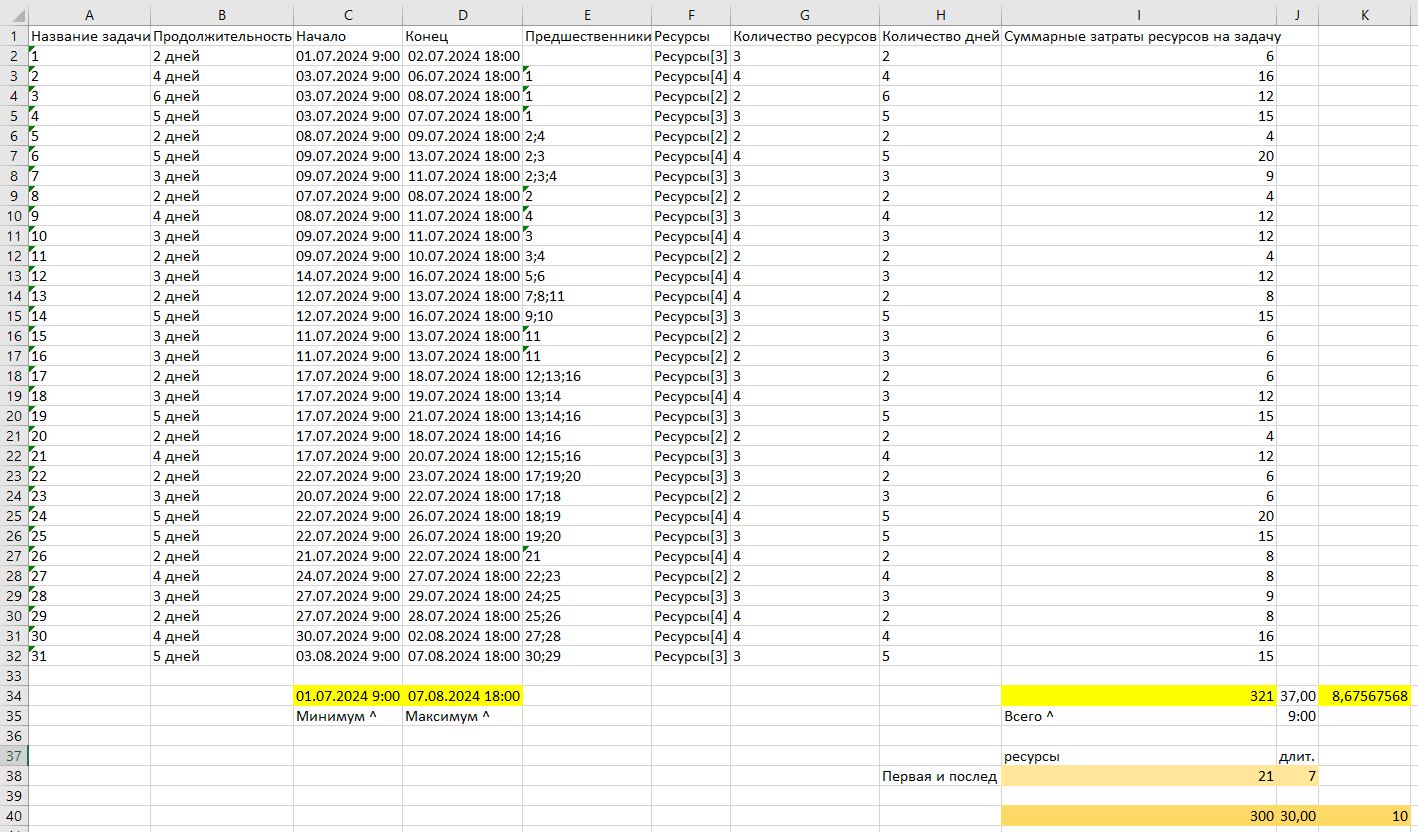
\includegraphics[width=\textwidth]{../img/init_time_estimation.png}\\
	
	Эксперименты:\\
	\textbf{Передвинем }начало второй работы на 5 дней (с 3.06 на 8.06).\\
	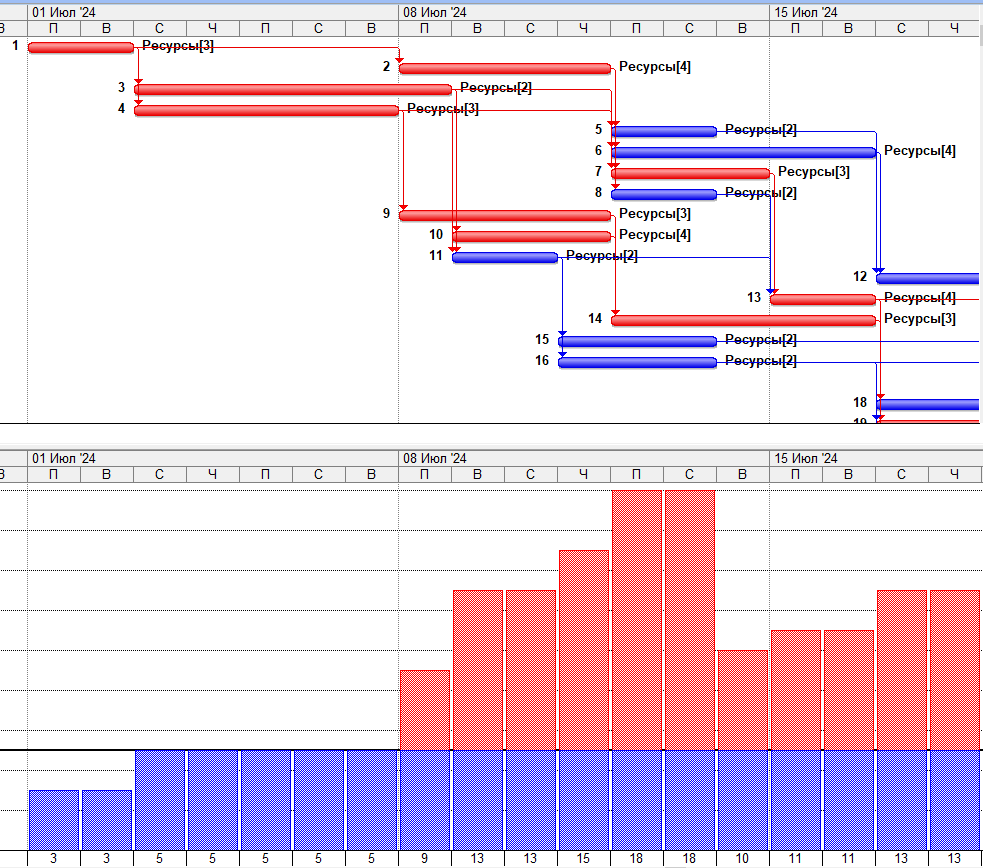
\includegraphics[width=0.5\textwidth]{../img/ot1a1_1.png}\\
	Теперь вторая работа тоже лежит на критичеком пути, значит правее её двигать нельзя.\\
	Теперь до 7.06 включительно тратится не более 5-ти ресурсов.\\
	На 8.06 есть 3 работы на критическом пути, сумма ресурсов которых равна 9.\\
	Значит без уменьшения длительности не обойтись.\\
	Чтобы уменьшить общее количество потраченных ресурсов как можно сильнее,
		нужно сократить длительность самой ресурсозатратной задачи.\\
	Из тех, что заканчиваются раньше 8.06 это задача №4\\
	\textbf{Уменьшим} длительность четвёртой работы на 2 дня (с 5 до 3).\\
	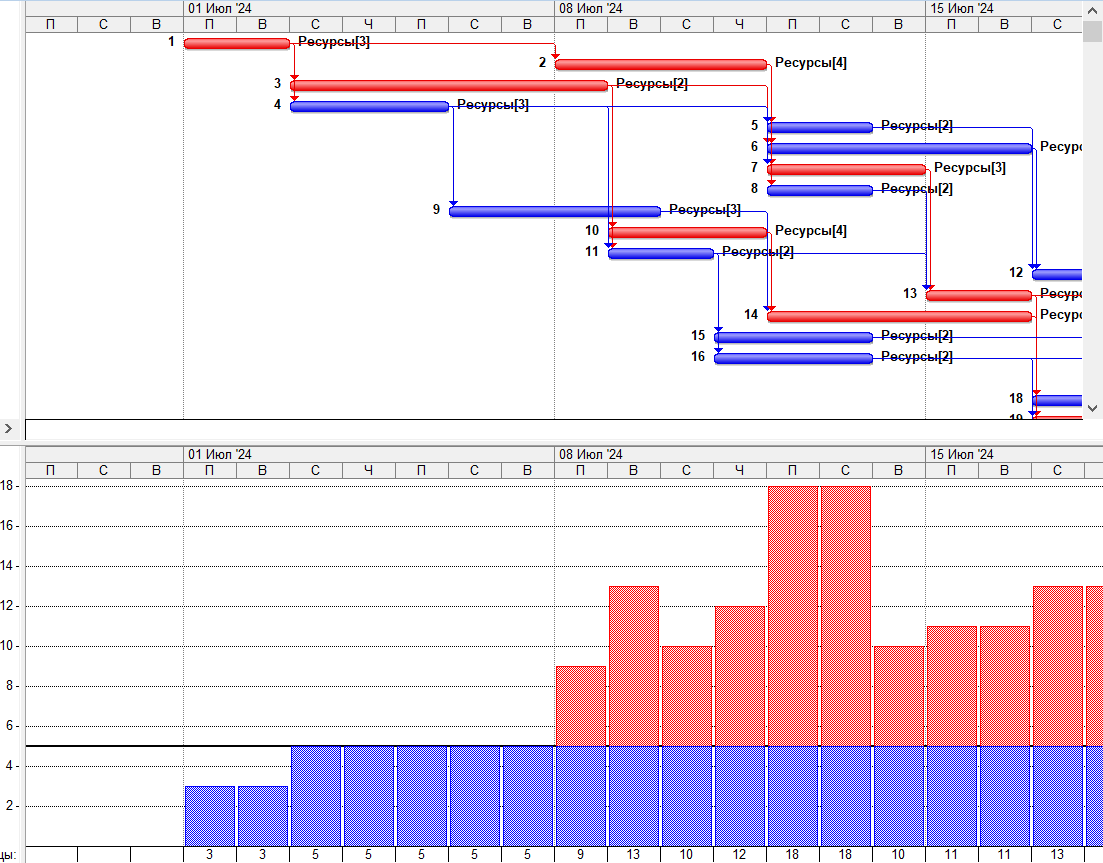
\includegraphics[width=0.3\textwidth]{../img/ot1a1_2.png}\\
	Внешне картина графика ресурсов не поменялся не поменялся.\\
	Это из-за того, что сразу после задачи №4 идёт задача №9 с таким же количеством ресурсов.\\
	Раз картина такая же, то можно, применить ту же логику и \textbf{уменьшить} длительность работы №9.\\
	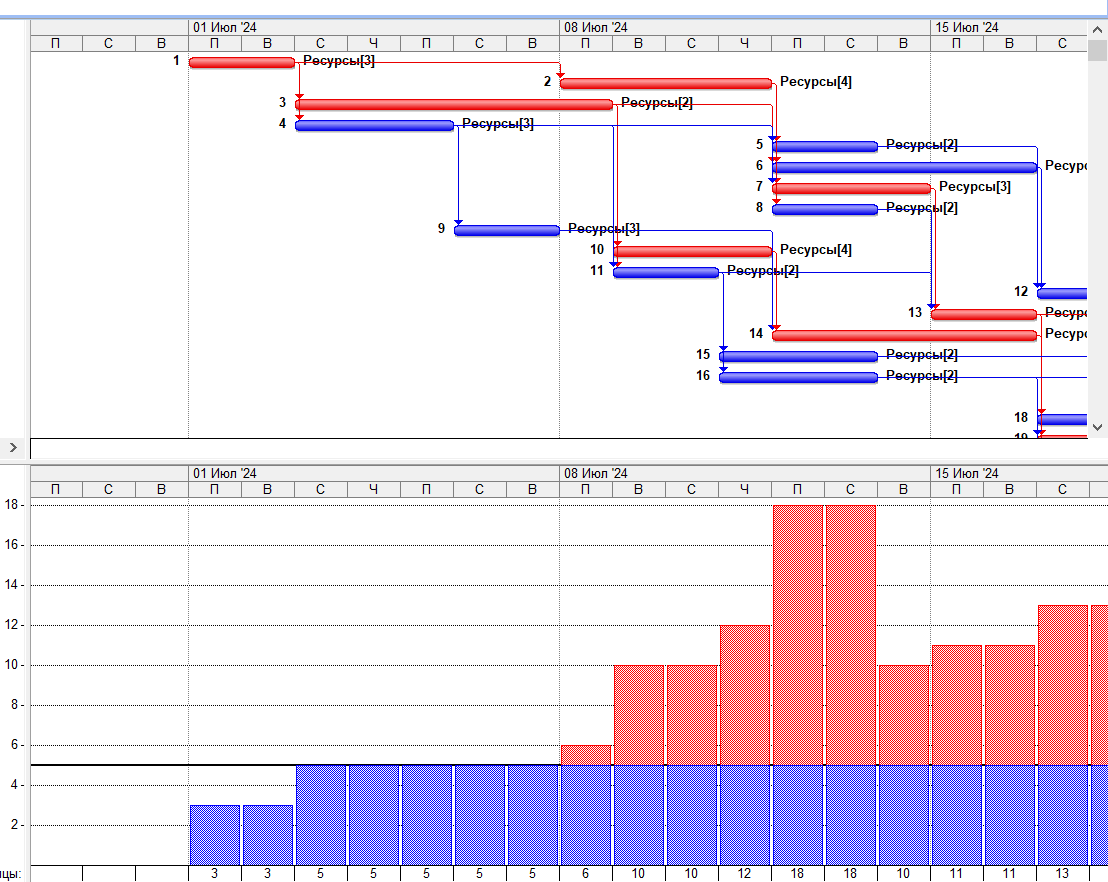
\includegraphics[width=0.5\textwidth]{../img/ot1a1_3.png}\\
	На 8.06 сейчас тратится на 1 ресурс больше, чем необходимо.
	В таком случае достаточно \textbf{уменьшить} длительноть задачи №3 на 1 день.\\ \
	[Возможность ветвиться: убрать 1 день или 2 дня от зад.№3]\\
	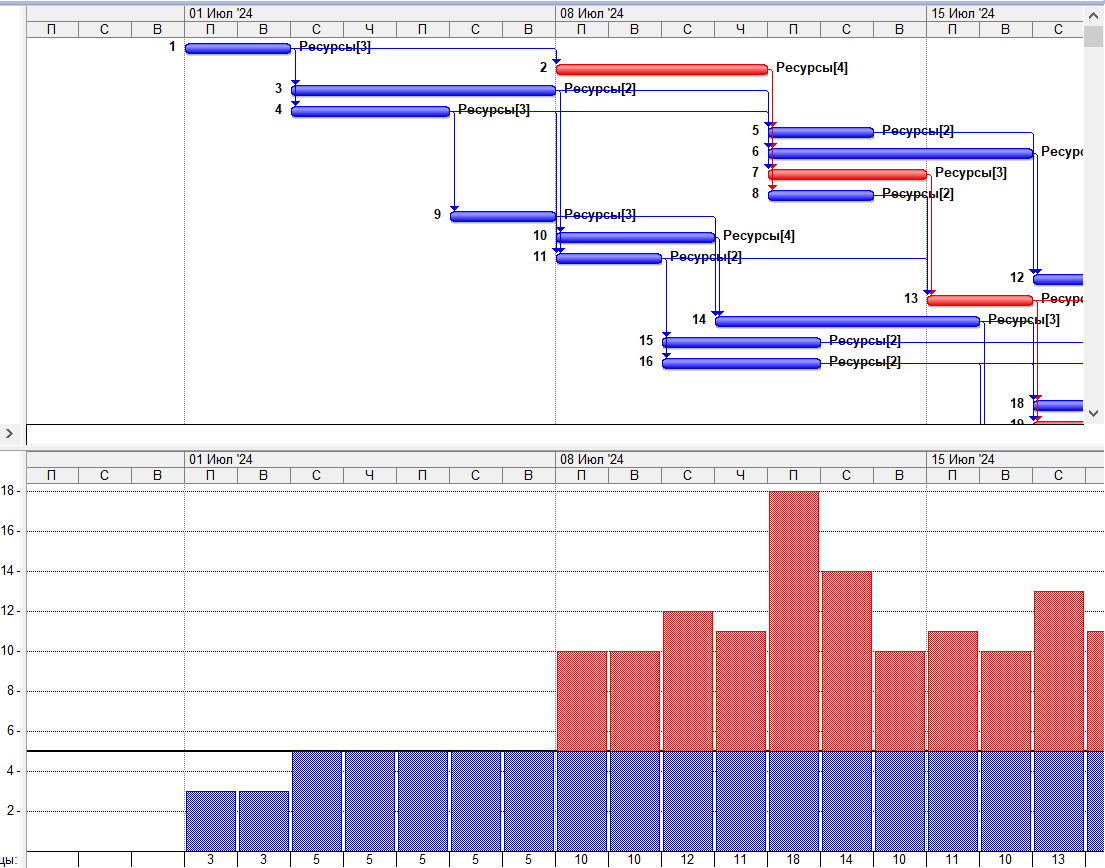
\includegraphics[width=0.5\textwidth]{../img/ot1a1_4.png}\\
	Задача №2 тратит 4 единицы ресурса в день.
	Раз в проекте нет задач, которые тратят 1 ресурс / день, то задача №2
		не может выполняться параллельно с какой-нибудь другой задачей.
	Тогда уменьшим длительность второй задачи на 1 день (с 4 на 3) и сдвинем задачи №10 и №11 впаво на 4 дня (с 08.06 на 12.06)\\
	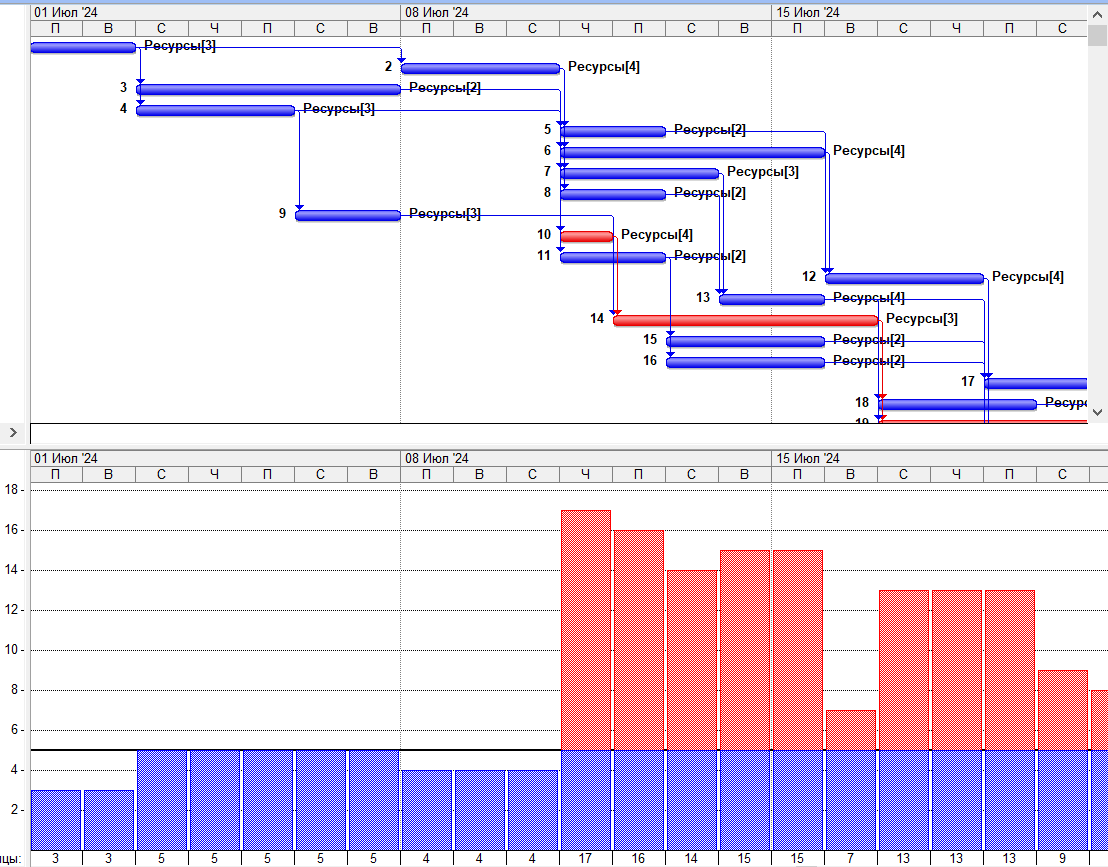
\includegraphics[width=0.5\textwidth]{../img/ot1a1_5.png}\\
\end{document}
